\documentclass{article}\usepackage[]{graphicx}\usepackage[]{color}
%% maxwidth is the original width if it is less than linewidth
%% otherwise use linewidth (to make sure the graphics do not exceed the margin)
\makeatletter
\def\maxwidth{ %
  \ifdim\Gin@nat@width>\linewidth
    \linewidth
  \else
    \Gin@nat@width
  \fi
}
\makeatother

\definecolor{fgcolor}{rgb}{0.345, 0.345, 0.345}
\newcommand{\hlnum}[1]{\textcolor[rgb]{0.686,0.059,0.569}{#1}}%
\newcommand{\hlstr}[1]{\textcolor[rgb]{0.192,0.494,0.8}{#1}}%
\newcommand{\hlcom}[1]{\textcolor[rgb]{0.678,0.584,0.686}{\textit{#1}}}%
\newcommand{\hlopt}[1]{\textcolor[rgb]{0,0,0}{#1}}%
\newcommand{\hlstd}[1]{\textcolor[rgb]{0.345,0.345,0.345}{#1}}%
\newcommand{\hlkwa}[1]{\textcolor[rgb]{0.161,0.373,0.58}{\textbf{#1}}}%
\newcommand{\hlkwb}[1]{\textcolor[rgb]{0.69,0.353,0.396}{#1}}%
\newcommand{\hlkwc}[1]{\textcolor[rgb]{0.333,0.667,0.333}{#1}}%
\newcommand{\hlkwd}[1]{\textcolor[rgb]{0.737,0.353,0.396}{\textbf{#1}}}%
\let\hlipl\hlkwb

\usepackage{framed}
\makeatletter
\newenvironment{kframe}{%
 \def\at@end@of@kframe{}%
 \ifinner\ifhmode%
  \def\at@end@of@kframe{\end{minipage}}%
  \begin{minipage}{\columnwidth}%
 \fi\fi%
 \def\FrameCommand##1{\hskip\@totalleftmargin \hskip-\fboxsep
 \colorbox{shadecolor}{##1}\hskip-\fboxsep
     % There is no \\@totalrightmargin, so:
     \hskip-\linewidth \hskip-\@totalleftmargin \hskip\columnwidth}%
 \MakeFramed {\advance\hsize-\width
   \@totalleftmargin\z@ \linewidth\hsize
   \@setminipage}}%
 {\par\unskip\endMakeFramed%
 \at@end@of@kframe}
\makeatother

\definecolor{shadecolor}{rgb}{.97, .97, .97}
\definecolor{messagecolor}{rgb}{0, 0, 0}
\definecolor{warningcolor}{rgb}{1, 0, 1}
\definecolor{errorcolor}{rgb}{1, 0, 0}
\newenvironment{knitrout}{}{} % an empty environment to be redefined in TeX

\let\hlesc\hlstd \let\hlpps\hlstd \let\hllin\hlstd \let\hlslc\hlcom \let\hlppc\hlcom
\usepackage{alltt}
\usepackage{natbib}
\usepackage[unicode=true]{hyperref}
\usepackage{geometry}
\usepackage{hyperref}
\usepackage{color}
\usepackage{amsmath}
\usepackage{amssymb}
\usepackage{verbatim}
\usepackage{mathpazo}
\usepackage{setspace}
\usepackage{multirow}
\usepackage{fullpage}
\usepackage{lscape}
\usepackage{fancyhdr}
\usepackage{wrapfig,lipsum,booktabs}
\usepackage[normalem]{ulem}
\usepackage[parfill]{parskip}
\usepackage{multirow}
\geometry{tmargin=1in,bmargin=1in,lmargin=1in,rmargin=1in}

\bibliographystyle{ecology_let}

%% for inline R code: if the inline code is not correctly parsed, you will see a message
\newcommand{\rinline}[1]{SOMETHING WRONG WITH knitr}


\IfFileExists{upquote.sty}{\usepackage{upquote}}{}
\begin{document}
\title{Proximity of restored hedgerows interacts with local floral diversity and species traits to shape  long-term pollinator metacommunity dynamics: a walk through of the models and analyses}
\author{Lauren Ponisio}


\maketitle

\begin{figure}[h!]
\centering
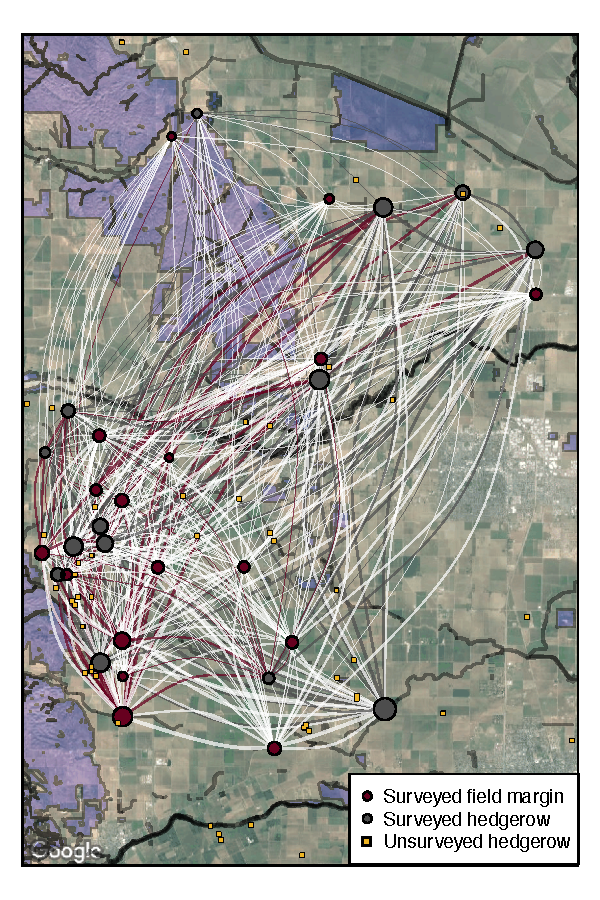
\includegraphics[width=0.6\textwidth]{figure/degree_spatial.pdf}
\label{fig:network}
\end{figure}
\clearpage

\section{Overview}
In our study we examine the metacommunity dynamics of plant-pollinator
communities using variety of different methods including 1) occupancy
modeling and 2) network analyses.  We are committed to reproducible
science and all analytical code will be maintained on github, along
with this write up.

The entire analysis is executable from the main.sh file. All of the
packages needed to run the analyses are listed in the packages.sh
file. All analyses were run using R (version $3.5.1$)
and nimble (0.6-12).

Note, there is an incompatibility with Nimble version 7.0 released in
February 2019. If this effects you can you either install the older
version of Nimble, or install from the branch
"avoid-protect-stack-overflow" directly from github. See post at
\url{https://groups.google.com/forum/#!topic/nimble-users/k6VMapOfxOk}

Hopefully this bug will be fixed soon and the models will run on any
version of NIMBLE.

Navigate to the analysis folder within the github repo
(hedgerow\_metacommunity) then the main.sh file can be selected and
run (a warning, the occupancy analyses each take several hours on my
2.3 GHz imac pro, so all together they will take quite a while), you
could run all of the analyses in the study by running this line in
BASH.

\begin{knitrout}
\definecolor{shadecolor}{rgb}{0.969, 0.969, 0.969}\color{fgcolor}\begin{kframe}
\noindent
\ttfamily
\hlstd{bash\ main.sh}\hspace*{\fill}
\mbox{}
\normalfont
\end{kframe}
\end{knitrout}

This will somewhat helpfully print the results of each analysis
and re-create any accompanying figures.

We will walk through each the main script for each analysis
individually.

\section{Occupancy model}

The occupancy models are run through the main.R file in the
analysis/occupancy folder. The script begins by setting the arguments
for prepping the data. Run as is to reproduce the data used in the
study. Prior analyses used the area of hedgerows in buffers weighted
by log distance from a focal site instead of the Gaussian decay
method, with similar results. In addition, the method for calculating
the habitat quality of a patch can be toggled using the
``col.name.div.type" argument. Other options are plant richness
``Richness" or the diversity of flowers visited by pollinators
``div.visits". All measures gave qualitatively similar results.

Importantly, ``natural.decay" and ``HR.decay" change the decay
($\alpha$) of weighting of remnant and hedgerow area,
respectively. Different combinations ($350$, $1000$, and $2500$) can
be used to change the steepness of the decay rate from very steep
($\alpha=350$ represents $98.5\%$ reduction in weight by $1$ $km$) to
very shallow ($\alpha=2500$ represents a $98.5\%$ reduction in weight
by $7$ $km$).


 The main.sh script executes all combinations of decay
rates. They are executed individually because the nimble models take a
considerable amount of computer memory which is not cleared after the
model is run. Running them all in a four loop within the same instance
of R would overload most computers. The last argument supplied is a
scale parameter to determine the number for iterations ($1e3$*scale)
and burnin ($1e1$*scale).

To run the MCMC in order to estimate the model coefficients, we use the
NIMBLE R package \citep{nimble-14, de2017programming}.  ``nimble"
stands for ``numerical inference for statistical models with Bayesian
and likelihood estimation."  It implements almost the same model
language as BUGS and JAGS, but supports easy customization of MCMC
algorithms, including writing new samplers, and user-defined functions
and distributions, which opens up enormous flexibility in how models
are written. This enabled us to integrate over the latent states,
increasing computational efficiency by an order of magnitude in
comparison to sampling every latent state. 


The multi-species, multi-season occupancy model is as follows (the
model code follows the notation in equation 5-6 in the manuscript,
except $HRwtProx$ is abbreviated as $hr.area$, and $RemnantWtProx$ as
$nat.area$):


\begin{knitrout}
\definecolor{shadecolor}{rgb}{0.969, 0.969, 0.969}\color{fgcolor}\begin{kframe}
\begin{alltt}
\hlstd{ms.ms.occ}
\end{alltt}
\begin{verbatim}
## {
##     mu.p.0 ~ dnorm(0, 0.001)
##     mu.p.day.1 ~ dnorm(0, 0.001)
##     mu.p.day.2 ~ dnorm(0, 0.001)
##     sigma.p.0 ~ dunif(0, 100)
##     sigma.p.day.1 ~ dunif(0, 100)
##     sigma.p.day.2 ~ dunif(0, 100)
##     mu.phi.0 ~ dnorm(0, 0.001)
##     mu.gam.0 ~ dnorm(0, 0.001)
##     sigma.phi.0 ~ dunif(0, 100)
##     sigma.gam.0 ~ dunif(0, 100)
##     mu.phi.hr.area ~ dnorm(0, 0.001)
##     mu.gam.hr.area ~ dnorm(0, 0.001)
##     sigma.phi.hr.area ~ dunif(0, 100)
##     sigma.gam.hr.area ~ dunif(0, 100)
##     mu.phi.nat.area ~ dnorm(0, 0.001)
##     mu.gam.nat.area ~ dnorm(0, 0.001)
##     sigma.phi.nat.area ~ dunif(0, 100)
##     sigma.gam.nat.area ~ dunif(0, 100)
##     mu.phi.fra ~ dnorm(0, 0.001)
##     mu.gam.fra ~ dnorm(0, 0.001)
##     sigma.phi.fra ~ dunif(0, 100)
##     sigma.gam.fra ~ dunif(0, 100)
##     phi.k ~ dnorm(0, 0.001)
##     gam.k ~ dnorm(0, 0.001)
##     gam.B ~ dnorm(0, 0.001)
##     phi.hr.area.fra ~ dnorm(0, 0.001)
##     gam.hr.area.fra ~ dnorm(0, 0.001)
##     phi.nat.area.fra ~ dnorm(0, 0.001)
##     gam.nat.area.fra ~ dnorm(0, 0.001)
##     phi.hr.area.k ~ dnorm(0, 0.001)
##     gam.hr.area.k ~ dnorm(0, 0.001)
##     phi.nat.area.k ~ dnorm(0, 0.001)
##     gam.nat.area.k ~ dnorm(0, 0.001)
##     phi.hr.area.B ~ dnorm(0, 0.001)
##     gam.hr.area.B ~ dnorm(0, 0.001)
##     phi.nat.area.B ~ dnorm(0, 0.001)
##     gam.nat.area.B ~ dnorm(0, 0.001)
##     for (sp in 1:nsp) {
##         p.0[sp] ~ dnorm(mu.p.0, sd = sigma.p.0)
##         p.day.1[sp] ~ dnorm(mu.p.day.1, sd = sigma.p.day.1)
##         p.day.2[sp] ~ dnorm(mu.p.day.2, sd = sigma.p.day.2)
##         phi.0[sp] ~ dnorm(mu.phi.0, sd = sigma.phi.0)
##         gam.0[sp] ~ dnorm(mu.gam.0, sd = sigma.gam.0)
##         phi.hr.area[sp] ~ dnorm(mu.phi.hr.area, sd = sigma.phi.hr.area)
##         gam.hr.area[sp] ~ dnorm(mu.gam.hr.area, sd = sigma.gam.hr.area)
##         phi.nat.area[sp] ~ dnorm(mu.phi.nat.area, sd = sigma.phi.nat.area)
##         gam.nat.area[sp] ~ dnorm(mu.gam.nat.area, sd = sigma.gam.nat.area)
##         phi.fra[sp] ~ dnorm(mu.phi.fra, sd = sigma.phi.fra)
##         gam.fra[sp] ~ dnorm(mu.gam.fra, sd = sigma.gam.fra)
##     }
##     for (sp in 1:nsp) {
##         for (site in 1:nsite) {
##             for (yr in 1:nyear) {
##                 for (rep in 1:nrep[site, yr, sp]) {
##                   logit(p[site, yr, rep, sp]) <- p.0[sp] + p.day.1[sp] * 
##                     day[site, yr, rep, sp] + p.day.2[sp] * day.2[site, 
##                     yr, rep, sp]
##                 }
##             }
##             logit(phi.site.sp.mean[site, sp]) <- mean(phi[site, 
##                 1:(nyear - 1), sp])
##             logit(gam.site.sp.mean[site, sp]) <- mean(gam[site, 
##                 1:(nyear - 1), sp])
##             psi.1[site, sp] <- gam.site.sp.mean[site, sp]/(1 - 
##                 phi.site.sp.mean[site, sp] + gam.site.sp.mean[site, 
##                 sp])
##             psi[site, 1, sp] <- psi.1[site, sp]
##             for (yr in 1:(nyear - 1)) {
##                 phi[site, yr, sp] <- phi.0[sp] + phi.k * k[sp] + 
##                   phi.B * B[sp] + phi.hr.area[sp] * HRarea[site] + 
##                   phi.nat.area[sp] * natural[site] + phi.fra[sp] * 
##                   fra[site, yr] + phi.hr.area.fra * fra[site, 
##                   yr] * HRarea[site] + phi.nat.area.fra * fra[site, 
##                   yr] * natural[site] + phi.hr.area.k * k[sp] * 
##                   HRarea[site] + phi.nat.area.k * k[sp] * natural[site] + 
##                   phi.hr.area.B * B[sp] * HRarea[site] + phi.nat.area.B * 
##                   B[sp] * natural[site]
##                 gam[site, yr, sp] <- gam.0[sp] + gam.k * k[sp] + 
##                   gam.B * B[sp] + gam.hr.area[sp] * HRarea[site] + 
##                   gam.nat.area[sp] * natural[site] + gam.fra[sp] * 
##                   fra[site, yr] + gam.hr.area.fra * fra[site, 
##                   yr] * HRarea[site] + gam.nat.area.fra * fra[site, 
##                   yr] * natural[site] + gam.hr.area.k * k[sp] * 
##                   HRarea[site] + gam.nat.area.k * k[sp] * natural[site] + 
##                   gam.hr.area.B * B[sp] * HRarea[site] + gam.nat.area.B * 
##                   B[sp] * natural[site]
##             }
##         }
##     }
##     for (site in 1:nsite) {
##         for (sp in 1:nsp) {
##             X[site, 1:nyear, 1:max.nreps, sp] ~ dDynamicOccupancy(nrep = nrep[site, 
##                 1:nyear, sp], psi1 = psi[site, 1, sp], phi = expit(phi[site, 
##                 1:(nyear - 1), sp]), gamma = expit(gam[site, 
##                 1:(nyear - 1), sp]), p = p[site, 1:nyear, 1:max.nreps, 
##                 sp])
##         }
##     }
## }
\end{verbatim}
\end{kframe}
\end{knitrout}

For those of you familiar with working in BUGS or JAGS, the main
difference here is the call to 'dDynamicOccupancy'. This is the
function allows us to numerically integrate over sequences of latent
states to directly calculate model likelihoods, removing the need to
perform MCMC sampling of these latent variables.



\begin{knitrout}
\definecolor{shadecolor}{rgb}{0.969, 0.969, 0.969}\color{fgcolor}\begin{kframe}
\begin{alltt}
\hlstd{dDynamicOccupancy}
\end{alltt}
\begin{verbatim}
## function (x, nrep, psi1, phi, gamma, p, log = 0) 
## {
##     ProbOccNextTime <- psi1
##     ll <- 0
##     nyears <- nimDim(x)[1]
##     if (nyears >= 1) {
##         for (t in 1:nyears) {
##             if (nrep[t] > 0) {
##                 numObs <- sum(x[t, 1:nrep[t]])
##                 if (numObs < 0) {
##                   nimPrint("Error in dDynamicOccupancy: numObs < 0 but nrep[t] > 0\n")
##                   nimStop("Error in dDynamicOccupancy: numObs < 0 but nrep[t] > 0\n")
##                 }
##                 ProbOccAndCount <- ProbOccNextTime * exp(sum(dbinom(x[t, 
##                   1:nrep[t]], size = 1, p = p[t, 1:nrep[t]], 
##                   log = 1)))
##                 ProbUnoccAndCount <- (1 - ProbOccNextTime) * 
##                   (numObs == 0)
##                 ProbCount <- ProbOccAndCount + ProbUnoccAndCount
##                 ProbOccGivenCount <- ProbOccAndCount/ProbCount
##                 ll <- ll + log(ProbCount)
##                 if (t < nyears) 
##                   ProbOccNextTime <- ProbOccGivenCount * phi[t] + 
##                     (1 - ProbOccGivenCount) * gamma[t]
##             }
##             else {
##                 if (t < nyears) 
##                   ProbOccNextTime <- ProbOccNextTime * phi[t] + 
##                     (1 - ProbOccNextTime) * gamma[t]
##             }
##         }
##     }
##     if (log) 
##         return(ll)
##     else return(exp(ll))
## }
## <environment: 0x7f84b30c25c8>
\end{verbatim}
\end{kframe}
\end{knitrout}

The number of MCMC iterations, burnin, number of chains, etc. can be
toggled by changing the value of the scale object. This script will
also generate MCMC diagnostic figures ($src\_plotting/checkChains.R$),
interaction plots ($src\_plotting/plotInteractions.R$), and posterior
mean and credible internal plots and table ($src\_plotting/posteriorPlotting.R$).


\section{Metacommunity Network Analysis}

There are three versions of the metacommunity network analysis. The
first two follow the suggestion of an anonymous reviewer and use the
inferred latent states from the occupancy model to estimate the
presence/absence of a species at a site. The third uses the raw
data. The results are almost completely consistent between the options,
though some of the pvalues bounce between marginally significant and
significant. 

Unfortunately, the fancy work we did to integrate out the latent
states (i.e., filter) is not helpful here since we need to sample the latent states
in order to use them in this analysis. So we created an alternative
version of the model which run a bit more slowly but samples all of
the latent states. It also outputs a truly massive model output with
with all the samples of the Zs.

In the main.sh file, you can run this model but setting filtering
FALSE which is done by passing the argument "latent" into the setup
code. We use the alpha values for the best fitting model. 

\begin{knitrout}
\definecolor{shadecolor}{rgb}{0.969, 0.969, 0.969}\color{fgcolor}\begin{kframe}
\noindent
\ttfamily
\hlstd{Rscript\ analysis}\hlopt{/}\hlstd{occupancy}\hlopt{/}\hlstd{main.R\ }\hlstr{"2500"}\hlstd{\ }\hlstr{"350"}\hlstd{\ }\hlstr{"latent"}\hlstd{\ }\hlstr{"all"}\hlstd{\ }\hlnum{1}\hlstd{e2}\hspace*{\fill}
\mbox{}
\normalfont
\end{kframe}
\end{knitrout}

Once we have the Zs, we have two options for creating the networks
from which to calculate the centrality metrics for species and
sites. The first creates a posterior distribution of metrics but
taking a random sample of the MCMC samples for the Zs, building
networks for each sample, then calculating metrics for each
sample. The mean and SD of the posterior distribution of network
metrics is then calculated and used in weighted linear mixed models. 


This analysis can be run using the following line in the shell

\begin{knitrout}
\definecolor{shadecolor}{rgb}{0.969, 0.969, 0.969}\color{fgcolor}\begin{kframe}
\noindent
\ttfamily
\hlstd{Rscript\ analysis}\hlopt{/}\hlstd{networks}\hlopt{/}\hlstd{Znetwork\textunderscore posterior.R}\hspace*{\fill}
\mbox{}
\normalfont
\end{kframe}
\end{knitrout}


The second flavor of this analysis uses the probability a species is
present at a site as inferred from the MCMC samples by taking the mean
Z value across all samples. This probability is then used as a weight
when constructing the metacommunity networks. The metrics of those
weighted networks and then used in the same linear mixed models as the
above (except without weights).

That analysis can be executed using the following line in the shell. 
\begin{knitrout}
\definecolor{shadecolor}{rgb}{0.969, 0.969, 0.969}\color{fgcolor}\begin{kframe}
\noindent
\ttfamily
\hlstd{Rscript\ analysis}\hlopt{/}\hlstd{networks}\hlopt{/}\hlstd{Znetwork.R}\hspace*{\fill}
\mbox{}
\normalfont
\end{kframe}
\end{knitrout}


The last variety of this analysis uses the raw data which includes
species abundances. The data is not corrected for imperfect detection.
The 'spTempMets.R' file executes the network analyses. The user can
provide any network metrics taken by the function 'speciesLevel' in
the bipartite package.

This analysis can be run using the following line in the shell

\begin{knitrout}
\definecolor{shadecolor}{rgb}{0.969, 0.969, 0.969}\color{fgcolor}\begin{kframe}
\noindent
\ttfamily
\hlstd{Rscript\ analysis}\hlopt{/}\hlstd{networks}\hlopt{/}\hlstd{spTempMets.R}\hspace*{\fill}
\mbox{}
\normalfont
\end{kframe}
\end{knitrout}


All of these flavors results in the same inferences about the effect
of site and species traits on their metacommunity network roles. 


\clearpage
\bibliography{refs}
\clearpage


\end{document}
